\chapter{Metodyka modelowania i oceny modeli}
\label{chap:metodyka-modelowania}

W rozdziale przedstawiono metodykę budowy i oceny modeli predykcyjnych. Problem badawczy sformułowano jako dwa odrębne zadania: klasyfikację binarną, czyli przewidywanie adopcji względem innych wyników, oraz regresję, czyli przewidywanie liczby dni do zakończenia pobytu. Zrezygnowano z analizy przeżycia (ang. \emph{survival analysis}) na rzecz prognozowania całkowitej długości pobytu (ang. \emph{length of stay}). W rozdziale opisano podział zbioru, dobór algorytmów uczących oraz zastosowane metryki oceny. Omówiono również interpretację wyników z wykorzystaniem wartości SHAP oraz protokół badawczy służący zapewnieniu odtwarzalności obliczeń.

\begin{table}[htbp]
\centering
\caption{Etapy procesu modelowania i oceny}
\label{tab:etapy-procesu-modelowania}
\small
\begin{tabular}{|p{0.24\textwidth}|p{0.66\textwidth}|}
\hline
\rowcolor{LightGray}
\textbf{Etap badawczy} & \textbf{Działanie} \\
\hline
1. Przygotowanie cech & Wykorzystanie zbioru zdefiniowanego w rozdziale 3. Wykluczenie atrybutów rejestrowanych po przyjęciu w celu uniknięcia wycieku informacji (ang. \emph{data leakage}). \\
\hline
2. Podział danych & Podział chronologiczny: zbiór treningowy (2013--2021), walidacyjny (2022--2023) oraz testowy (2024--2025). \\
\hline
3. Uczenie modeli & Trenowanie modeli bazowych i zespołowych osobno dla klasyfikacji i regresji. \\
\hline
4. Ocena modeli & Ocena klasyfikacji za pomocą AUC-ROC, AUC-PR, F1-Score oraz regresji za pomocą MAE, RMSE i MedAE. \\
\hline
5. Interpretacja & Analiza wyjaśnień globalnych i lokalnych za pomocą SHAP oraz wpływ zdefiniowanych Rodzin Cech. \\
\hline
6. Reprodukowalność & Deterministyczna inicjalizacja algorytmów (\texttt{random\_state=42}) oraz statyczny zapis wyników. \\
\hline
\end{tabular}
\end{table}

\section{Cel modelowania}
\label{sec:cel-modelowania}

Celem modelowania predykcyjnego jest prognozowanie wyników wyłącznie na podstawie informacji dostępnych w momencie przyjęcia zwierzęcia do schroniska. Analiza koncentruje się na mocy predykcyjnej modeli, a nie na wnioskowaniu przyczynowo-skutkowym.

Modele mają określić, w jakim stopniu atrybuty takie jak gatunek, kategoria wiekowa czy okoliczności przyjęcia pozwalają przewidzieć dwie wartości: (1) prawdopodobieństwo adopcji zwierzęcia oraz (2) całkowity czas zajmowania miejsca w schronisku do momentu zakończenia pobytu, na przykład adopcji, transferu lub powrotu do właściciela. Takie podejście dostarcza prognoz, które mogą być przydatne w zarządzaniu placówką, ponieważ czas pobytu każdego zwierzęcia wiąże się z kosztami operacyjnymi.

\section{Formalne sformułowanie problemu}
\label{sec:formalne-sformulowanie-problemu}

Modele uczono dla dwóch zadań:

\begin{enumerate}\itemsep2pt
\item \textbf{Klasyfikacja binarna (\texttt{classification\_target}):} zmienna objaśniana $Y^{(kl)} \in \{0,1\}$, gdzie $Y^{(kl)}=1$ oznacza adopcję, a $Y^{(kl)}=0$ inny wynik końcowy. Szacowane jest prawdopodobieństwo adopcji $P(Y^{(kl)}=1\mid X)$.
\item \textbf{Regresja długości pobytu (\texttt{regression\_target\_days}):} zmienna ciągła wyrażona w dobach, reprezentująca czas do zdarzenia kończącego pobyt. Model estymuje wartość oczekiwaną długości trwania epizodu $E(T\mid X)$.
\end{enumerate}

Nie zastosowano modeli analizy przeżycia, takich jak model proporcjonalnych hazardów Coxa czy Random Survival Forest. Wymagałoby to bardziej złożonej estymacji w obecności cenzurowania prawostronnego. Uczenie predykcyjne zdefiniowano jako klasyczną regresję na zamkniętych pobytach, dla których długość pobytu można zmierzyć bezpośrednio.

Zbiór predyktorów $X$ nie zawiera cech będących składową wyniku końcowego.

\section{Przygotowanie danych i podział chronologiczny}
\label{sec:przygotowanie-danych-podzial}

Dane mają charakter czasowy, dlatego zrezygnowano z klasycznej walidacji krzyżowej (ang. \emph{k-fold cross-validation}) z tasowaniem próbek. Celem było uniknięcie wycieku informacji. Uczenie modelu na późniejszych rocznikach i testowanie go na wcześniejszych mogłoby zawyżyć ocenę skuteczności, ponieważ model korzystałby pośrednio z późniejszych wzorców.

Zbiór 162 390 epizodów podzielono chronologicznie na trzy części:

\begin{itemize}\itemsep2pt
\item \textbf{Zbiór treningowy:} lata 2013--2021. Pula obejmująca 126 759 rekordów psów i kotów.
\item \textbf{Zbiór walidacyjny:} lata 2022--2023. Obejmuje 21 811 epizodów. Przeznaczony do doboru parametrów modeli i wskaźników odcięcia.
\item \textbf{Zbiór testowy:} lata 2024--2025. Obejmuje 13 820 epizodów. Służy wyłącznie do ostatecznej oceny najlepszych algorytmów na najnowszych danych.
\end{itemize}

\begin{figure}[htbp]
\centering
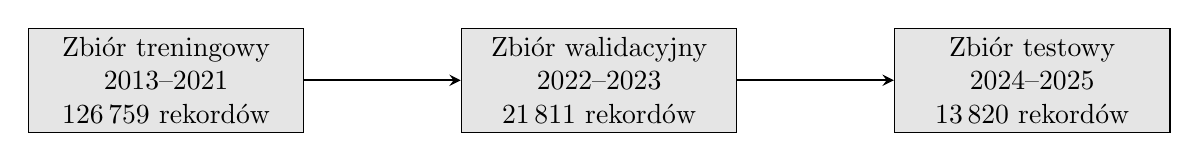
\begin{tikzpicture}[
    box/.style={draw, rectangle, minimum width=3.5cm, minimum height=1.2cm, align=center, fill=black!10},
    arrow/.style={thick, ->, >=stealth}
]
\node[box] (train) at (0,0) {Zbiór treningowy\\2013--2021\\126\,759 rekordów};
\node[box] (val) at (5.5,0) {Zbiór walidacyjny\\2022--2023\\21\,811 rekordów};
\node[box] (test) at (11,0) {Zbiór testowy\\2024--2025\\13\,820 rekordów};
\draw[arrow] (train) -- (val);
\draw[arrow] (val) -- (test);
\end{tikzpicture}
\caption{Chronologiczny podział zbioru danych}
\label{fig:podzial-chronologiczny}
\end{figure}

Taki podział pozwala ocenić odporność modelu na zmiany wzorców w czasie (ang. \emph{concept drift}), zwłaszcza w okresie po pandemii COVID-19.

\section{Algorytmy predykcyjne}
\label{sec:algorytmy-predykcyjne}

W badaniu porównano proste modele odniesienia z bardziej zaawansowanymi algorytmami zespołowymi. Pozwala to ocenić, czy zastosowanie bardziej złożonych metod poprawia jakość predykcji.

\textbf{Modele bazowe:}

\begin{itemize}\itemsep2pt
\item \textbf{Modele odniesienia (Dummy):} przewidują klasę większościową w klasyfikacji lub medianę w regresji. Wyznaczają minimalny poziom odniesienia dla oceny błędu w ujęciu deterministycznym.
\item \textbf{Modele liniowe:} regresja logistyczna dla binarnej zmiennej celu oraz regresja grzbietowa (Ridge) dla regresji długości pobytu. Zapewniają stabilność wyników i umożliwiają stosunkowo prostą analizę wag atrybutów. Prawdopodobieństwo w modelu regresji logistycznej wyraża się wzorem:
\begin{equation}
P(Y=1|X) = \frac{1}{1 + e^{-(\beta_0 + \beta_1 X_1 + \dots + \beta_p X_p)}}
\end{equation}
\end{itemize}

\textbf{Modele zaawansowane (drzewa decyzyjne):}

\begin{itemize}\itemsep2pt
\item \textbf{Lasy Losowe (Random Forest, \cite{Breiman2001}):} model zespołowy łączący predykcje $T$ drzew decyzyjnych, każde uczone na losowym podzbiorze obserwacji (ang.\ \emph{bagging}) i losowym podzbiorze $\sqrt{p}$ spośród $p$ cech. Agregacja przez uśrednianie (regresja) lub głosowanie większościowe (klasyfikacja) istotnie redukuje wariancję w porównaniu z pojedynczym drzewem. RF nie wymaga skalowania predyktorów, lecz wymaga jawnego kodowania zmiennych kategorycznych.
\item \textbf{Histogram-based Gradient Boosting (HistGB, \cite{Ke2017,Friedman2001}):} wariant sekwencyjnego uczenia na pseudoresztkach, gdzie każde kolejne drzewo koryguje błędy poprzedniego. Kluczową innowacją jest dyskretyzacja predyktorów numerycznych do histogramów ($\leq 255$ kubełków), co skraca złożoność uczenia. Algorytm obsługuje brakujące wartości natywnie i nie wymaga skalowania ani imputacji.
\item \textbf{CatBoost \cite{Prokhorenkova2018}:} architektura z rodziny wzmacniania gradientowego (ang. \emph{Gradient Boosting}). Zawiera mechanizmy przetwarzania zmiennych kategorycznych bez konieczności sztucznej wektoryzacji (\emph{one-hot encoding}). Z tego powodu dobrze nadaje się do danych zawierających setki nominalnych wartości ras i umaszczeń zwierząt. Ogólna funkcja celu minimalizowana w kolejnych iteracjach algorytmów z tej rodziny ma postać:
\begin{equation}
\mathcal{L}^{(t)} = \sum_{i=1}^n l(y_i, \hat{y}_i^{(t-1)} + f_t(x_i)) + \Omega(f_t)
\end{equation}
gdzie $l$ to różniczkowalna funkcja straty, $\hat{y}_i^{(t-1)}$ to predykcja z poprzedniej iteracji, $f_t$ to nowo dodawane drzewo, a $\Omega(f_t)$ to człon regularyzacyjny~\cite{Friedman2001}.
\end{itemize}

\begin{table}[htbp]
\centering
\caption{Porównanie wykorzystanych rodzin algorytmów predykcyjnych}
\label{tab:algorytmy-porownanie}
\small
\begin{tabular}{|l|c|c|p{4cm}|}
\hline
\rowcolor{LightGray}
\textbf{Algorytm} & \textbf{Obsługa zm. kategorycznych} & \textbf{Nieliniowość} & \textbf{Główne zastosowanie} \\
\hline
Dummy & Brak & Nie dotyczy & Punkt odniesienia (ang. \emph{baseline}) \\
\hline
Logistic/Ridge Regression & Wymaga wektoryzacji & Nie & Stabilne modele liniowe \\
\hline
Random Forest & Wymaga wektoryzacji & Tak & Algorytm zespołowy redukujący wariancję \\
\hline
HistGradientBoosting & Natywna & Tak & Szybkie trenowanie dla dużych zbiorów \\
\hline
CatBoost & Natywna, zaawansowana & Tak & Główne modele, wysoka skuteczność dla cech nominalnych \\
\hline
\end{tabular}
\end{table}

Dla danych tabelarycznych z dużą liczbą zmiennych kategorycznych wybrano modele oparte na drzewach decyzyjnych (\emph{gradient boosting}). Decyzja ta wynika z tego, że algorytmy te są często uznawane za jeden ze standardów dla tego typu danych (ang. \emph{state-of-the-art})~\cite{Grinsztajn2022}. W przeciwieństwie do modeli liniowych, dobrze wychwytują nieliniowe interakcje między zmiennymi, na przykład specyficzny wpływ wieku tylko u konkretnej rasy psów, i nie wymagają rygorystycznego skalowania danych numerycznych.

Zrezygnowano z zastosowania głębokich sieci neuronowych (ang. \emph{Deep Learning}). Literatura badawcza i praktyka inżynieryjna wskazują, że sieci neuronowe często nie poprawiają jakości estymacji na niejednorodnych zbiorach tabelarycznych w porównaniu z algorytmami z rodziny \emph{gradient boosting}. Jednocześnie wymagają większych zasobów obliczeniowych i ograniczają łatwość interpretacji wyników, co określa się często jako problem czarnej skrzynki.

W procesie strojenia modeli, szczególnie CatBoost, przyjęto zachowawczą strategię doboru hiperparametrów, aby ograniczyć ryzyko przeuczenia (ang. \emph{overfitting}). Zastosowano umiarkowaną głębokość drzew decyzyjnych (\texttt{depth=6}), co ogranicza zapamiętywanie szumu z danych treningowych, oraz niski współczynnik uczenia (\texttt{learning\_rate=0.05}), pozwalający na stopniową i stabilną zbieżność algorytmu w trakcie 1000 iteracji. Dodatkowym mechanizmem kontrolnym było wczesne zatrzymywanie (\texttt{early\_stopping\_rounds=50}), które automatycznie przerywało proces uczenia, gdy metryka na zbiorze walidacyjnym przestawała się poprawiać.

\begin{table}[htbp]
\centering
\caption{Wybrane hiperparametry dla modeli wzmacniania gradientowego}
\label{tab:hiperparametry}
\small
\begin{tabular}{|l|l|l|}
\hline
\rowcolor{LightGray}
\textbf{Algorytm} & \textbf{Parametr} & \textbf{Wartość} \\
\hline
CatBoost & \texttt{depth} & 6 \\
 & \texttt{learning\_rate} & 0.05 \\
 & \texttt{iterations} & 1000 \\
 & \texttt{early\_stopping\_rounds} & 50 \\
\hline
HistGradientBoosting & \texttt{max\_depth} & \texttt{None} \\
 & \texttt{learning\_rate} & 0.1 \\
\hline
\end{tabular}
\end{table}

\section{Metryki oceny}
\label{sec:metryki-oceny}

Zastosowano następujące metryki oceny:

\textbf{Zadanie klasyfikacji:}

\begin{itemize}\itemsep2pt
\item \textbf{AUC-ROC (Area Under the Receiver Operating Characteristic Curve, \cite{Fawcett2006}):} miara ogólnej zdolności modelu do rozróżniania klas. Wartość 1.0 oznacza idealne rozróżnianie, a 0.5 prognozę losową. Matematycznie można ją wyrazić jako prawdopodobieństwo, że model oceni wyżej losowo wybrany przypadek pozytywny niż negatywny:
\begin{equation}
\text{AUC-ROC} = P(\hat{p}_1 > \hat{p}_0)
\end{equation}
\item \textbf{AUC-PR (Area Under the Precision-Recall Curve):} metryka przydatna przy niewielkiej nierównowadze klas, opisująca skuteczność wykrywania kluczowej klasy~\cite{Davis2006}. Precyzja i czułość zdefiniowane są jako:
\begin{equation}
\text{Precision} = \frac{TP}{TP + FP}, \qquad \text{Recall} = \frac{TP}{TP + FN}
\end{equation}
AUC-PR stanowi pole pod krzywą Precision--Recall wyznaczoną dla wszystkich możliwych progów odcięcia. W przeciwieństwie do AUC-ROC, ignoruje przypadki prawdziwie negatywne, co czyni ją bardziej wrażliwą na jakość wykrywania klasy mniejszościowej~\cite{Davis2006}.
\item \textbf{F1-Score, precyzja (Precision) i czułość (Recall):} miary punktowe zależne od wyboru progu odcięcia (ang. \emph{threshold}). Miara F1 jest średnią harmoniczną precyzji i czułości:
\begin{equation}
F_1 = 2 \cdot \frac{\text{Precision} \cdot \text{Recall}}{\text{Precision} + \text{Recall}}
\end{equation}
W metodyce pracy zrezygnowano z naiwnego wyboru progu \texttt{0.5}. Optymalny próg decyzyjny dla każdego algorytmu został dobrany na niezależnym zbiorze walidacyjnym pod kątem maksymalizacji wskaźnika F1, a następnie zastosowany na zbiorze testowym w celu ewaluacji.
\item \textbf{Ocena kalibracji (Brier Score):} wysoki wynik AUC nie gwarantuje, że szacowane prawdopodobieństwa odpowiadają rzeczywistej częstości. Wynik Briera (ang.\ \emph{Brier Score}~\cite{Brier1950}) mierzy średni błąd kwadratowy:
\begin{equation}
\text{BS} = \frac{1}{n} \sum_{i=1}^{n} \left(p_i - o_i\right)^2
\label{eq:brier-score}
\end{equation}
gdzie $p_i \in [0,1]$ to prognozowane prawdopodobieństwo adopcji, a $o_i \in \{0,1\}$ to rzeczywisty wynik. Wartość $\text{BS} = 0$ odpowiada idealnej kalibracji~\cite{NiculescuMizil2005}. W celu oceny kalibracji wygenerowano wykresy kalibracyjne. Jest to ważne z punktu widzenia budowy wiarygodnego narzędzia analitycznego dla personelu schroniska.
\end{itemize}

\textbf{Zadanie regresji:}

\begin{itemize}\itemsep2pt
\item \textbf{MAE (Mean Absolute Error):} średni błąd bezwzględny, mierzony w dniach. Jest to główna metryka oceniająca przeciętną pomyłkę modelu:
\begin{equation}
\text{MAE} = \frac{1}{n} \sum_{i=1}^n |y_i - \hat{y}_i|
\end{equation}
\item \textbf{MedAE (Median Absolute Error):} mediana błędów bezwzględnych. Jest to metryka odporna na błędy skrajne, na przykład przypadki zwierząt pozostających w schronisku latami.
\item \textbf{RMSE (Root Mean Square Error):} pierwiastek błędu średniokwadratowego. Metryka silniej penalizuje największe pomyłki modelu:
\begin{equation}
\text{RMSE} = \sqrt{\frac{1}{n} \sum_{i=1}^n (y_i - \hat{y}_i)^2}
\end{equation}
\end{itemize}

\section{Interpretowalność (SHAP)}
\label{sec:interpretowalnosc-shap}

Wyniki modeli predykcyjnych w kontekście schroniskowym i weterynaryjnym powinny być możliwie przejrzyste. Do analizy wpływu poszczególnych cech wykorzystano wartości SHAP (ang.\ \emph{SHapley Additive exPlanations})~\cite{Lundberg2017}.

Metoda ta wywodzi się z kooperatywnej teorii gier i pozwala oszacować wkład poszczególnych atrybutów w końcową prognozę modelu, wykorzystując wartości Shapleya określane wzorem:
\begin{equation}
\phi_j = \sum_{S \subseteq F \setminus \{j\}} \frac{|S|! (|F| - |S| - 1)!}{|F|!} \left[ f_x(S \cup \{j\}) - f_x(S) \right]
\end{equation}
gdzie $F$ to zbiór wszystkich cech, $S$ to podzbiór cech niezawierający cechy $j$, a $f_x(S)$ to prognoza dla podzbioru cech $S$.

\begin{enumerate}\itemsep2pt
\item \textbf{Wyjaśnienia globalne (SHAP Summary):} zestawienie pokazujące średni wpływ cech na decyzje modelu w całym zbiorze, na przykład związek młodego wieku z wyższym prawdopodobieństwem adopcji.
\item \textbf{Wyjaśnienia lokalne:} ocena znaczenia atrybutów w konkretnym pojedynczym epizodzie. Funkcja ta rozkłada prognozę na czynniki zwiększające lub zmniejszające końcowy wynik.
\item \textbf{Analiza Rodzin Cech:} atrybuty pogrupowano w ,,Rodziny Cech'', na przykład Wiek, Wygląd i Kontekst. Takie podejście umożliwia odrzucenie lub zachowanie wybranych grup zmiennych oraz sprawdzenie ogólnego spadku celności bez konieczności osobnego analizowania wpływu pojedynczych wektorów.
\end{enumerate}

\begin{figure}[htbp]
\centering
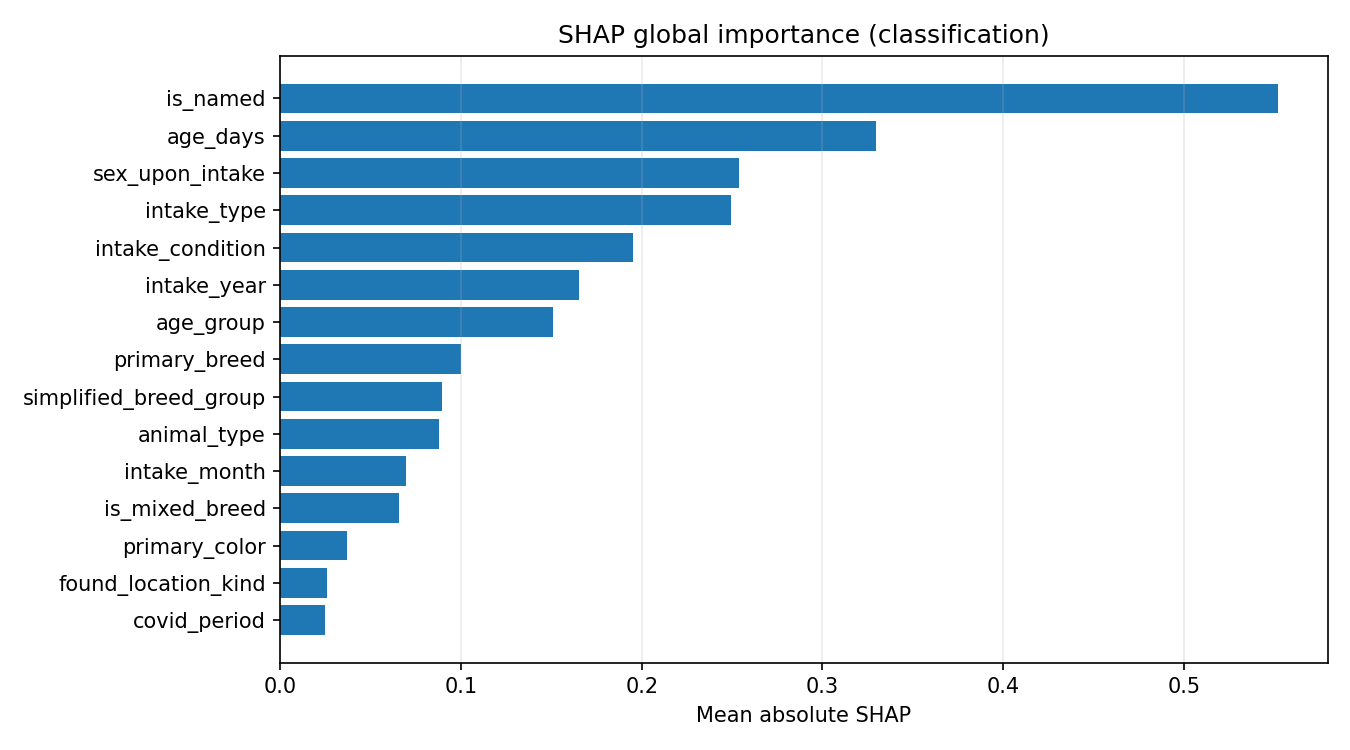
\includegraphics[width=0.90\textwidth]{../reports/figures/shap_summary_classification.png}
\caption{Wykres SHAP Summary (beeswarm) dla klasyfikatora adopcji~\cite{Lundberg2017}. Każdy punkt odpowiada jednej obserwacji ze zbioru testowego. Kolor odzwierciedla wartość cechy (czerwony -- wysoka, niebieski -- niska), a pozycja pozioma -- wartość SHAP. Szczegółowa interpretacja wyników w rozdziale~5.}
\label{fig:shap-summary-preview-ch4}
\end{figure}

\begin{figure}[htbp]
\centering
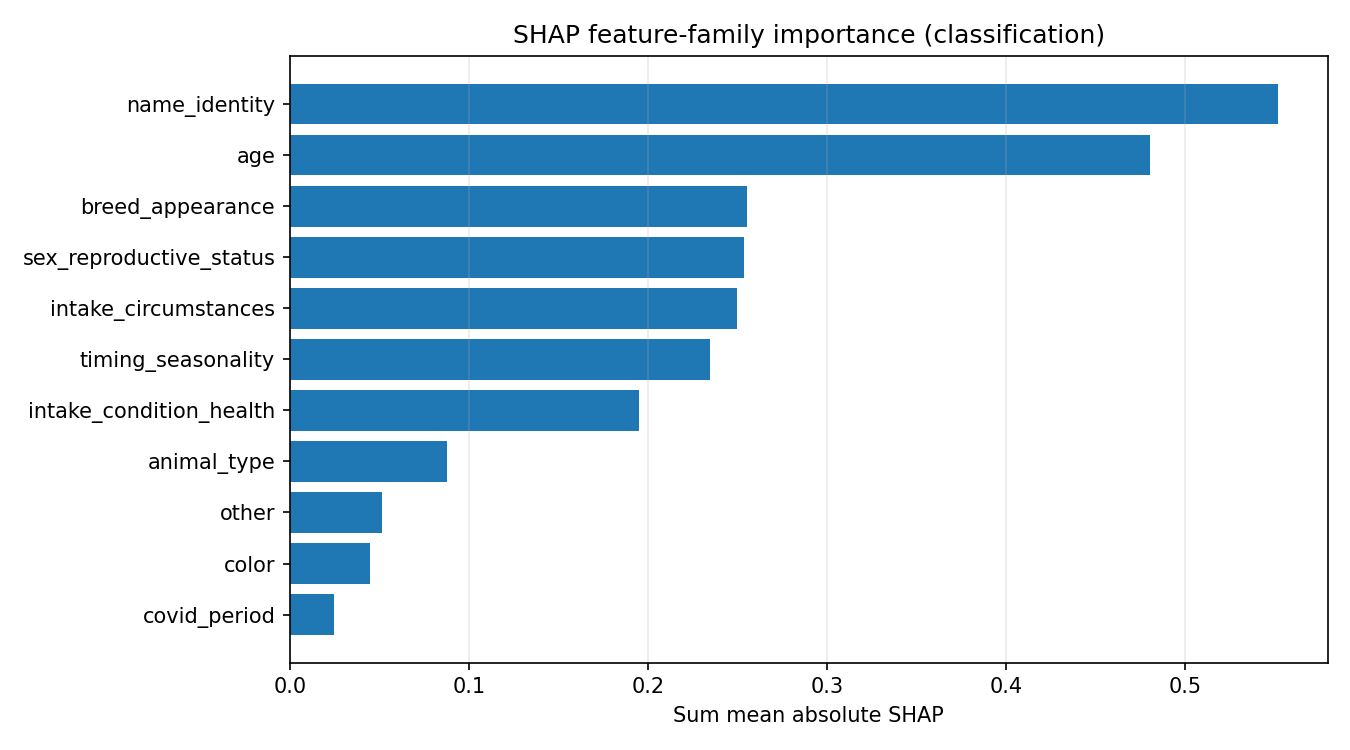
\includegraphics[width=0.90\textwidth]{../reports/figures/shap_feature_families_classification.png}
\caption{Zagregowany wpływ Rodzin Cech na predykcje klasyfikatora (suma bezwzględnych wartości SHAP per Rodzina). Grupowanie cech pozwala ocenić relatywny wkład całych kategorii atrybutów.}
\label{fig:shap-families-preview-ch4}
\end{figure}

\section{Protokół eksperymentu}
\label{sec:protokol-eksperymentu}

W celu zapewnienia odtwarzalności eksperymentu zastosowano następujące zasady:

\begin{enumerate}\itemsep2pt
\item \textbf{Jednolite ziarno losowości:} ustalono deterministyczne ziarno liczb pseudolosowych (\texttt{random\_state=42}) dla algorytmów.
\item \textbf{Rozdzielenie obliczeń i wizualizacji:} proces uczenia odbywa się poprzez dedykowany skrypt (\texttt{scripts/run\_full\_pipeline.py}).
\item \textbf{Zapis modeli:} wyniki modelowania i metadane ewaluacyjne zapisywane są bezpośrednio na dysk jako estymatory \texttt{.joblib} oraz tabele \texttt{.csv}. Interfejs analityczny jedynie odczytuje zapisane parametry, bez konieczności kosztownego ponownego uczenia modeli.
\end{enumerate}

Algorytm \ref{alg:protokol} przedstawia uproszczony pseudokod procesu uczenia i oceny, realizowany w ramach protokołu badawczego.

\begin{algorithm}[htbp]
\caption{Protokół treningu i oceny modelu}\label{alg:protokol}
\KwIn{Zbiór danych $D$, konfiguracje hiperparametrów $\Theta$}
\KwOut{Wytrenowane modele $M$, metryki oceny $E$}
\BlankLine
$D_{train} \gets$ podzbiór $D$ (lata 2013--2021)\;
$D_{val} \gets$ podzbiór $D$ (lata 2022--2023)\;
$D_{test} \gets$ podzbiór $D$ (lata 2024--2025)\;
\ForEach{zadanie $\in \{ \text{klasyfikacja}, \text{regresja} \}$}{
  \ForEach{algorytm $\in \{ \text{Dummy, Logistic/Ridge, RF, HistGB, CatBoost} \}$}{
    $M_{alg} \gets$ Inicjuj(algorytm, $\Theta_{alg}$, \texttt{random\_state}=42)\;
    Trenuj $M_{alg}$ na $D_{train}$ używając \texttt{early\_stopping} na $D_{val}$\;
    \If{zadanie == \text{klasyfikacja}}{
      Optymalizuj próg odcięcia dla metryki F1 na $D_{val}$\;
    }
    $\hat{y} \gets$ Prognozuj dla $D_{test}$ z modelem $M_{alg}$\;
    $E_{alg} \gets$ Oblicz metryki ewaluacyjne($\hat{y}$, $D_{test}$)\;
    Zapisz $M_{alg}$ (\texttt{.joblib}) oraz $E_{alg}$ (\texttt{.csv})\;
  }
}
Wyprowadź globalne i lokalne wartości SHAP dla modeli CatBoost\;
\end{algorithm}

\section{Ograniczenia}
\label{sec:ograniczenia-modelowania}

Zastosowane modele mają kilka ograniczeń. Głównym ograniczeniem technicznym było wykluczenie pobytów nieukończonych w momencie pobrania bazy, czyli obserwacji objętych cenzorowaniem prawostronnym. Było to konieczne do przeprowadzenia wariantu regresji długości pobytu.

Ponadto modele odzwierciedlają statystyczne uwarunkowania lokalnego rynku w określonym przedziale czasu, szczególnie zasady działania AAC jako schroniska no-kill o wskaźniku przeżycia powyżej 90\%. Prawidłowości przypisane na przykład do etykiet rasy mogą zależeć od lokalnej struktury społecznej i sposobu postrzegania zwierząt. Ich bezpośrednie przeniesienie do innych schronisk bez ponownego trenowania lub kalibracji mogłoby obniżyć skuteczność predykcyjną.